\documentclass[10pt,twoside]{article}

\usepackage[T1]{fontenc}
\usepackage[utf8]{inputenc}
\usepackage{newtxtext}
\usepackage{mathtools,amsthm}
\usepackage{newtxmath}
\usepackage[margin=0.78in,top=0.62in,bottom=0.70in]{geometry}
\usepackage{microtype}
\usepackage{xcolor}
\usepackage{booktabs,tabularx,array}
\usepackage{enumitem}
\usepackage{titlesec}
\usepackage{caption}
\usepackage{float}
\usepackage{tikz}
\usepackage{pgfplots}
\usepackage[numbers,sort&compress]{natbib}
\usepackage[colorlinks=true,allcolors=MidnightBlue]{hyperref}
\usepackage[nameinlink,noabbrev]{cleveref}

\pgfplotsset{compat=1.18}

\definecolor{MidnightBlue}{HTML}{16324F}
\definecolor{SignalBlue}{HTML}{277DA1}
\definecolor{WarmGold}{HTML}{D69E2E}
\definecolor{SoftRed}{HTML}{C8553D}
\definecolor{Forest}{HTML}{3D7A62}
\definecolor{Ink}{HTML}{20262E}
\definecolor{Mist}{HTML}{F2F5F7}
\definecolor{RuleGray}{HTML}{CBD5DE}

\color{Ink}
\hypersetup{pdfauthor={Jonathan R. Landers},pdftitle={Prediction Is Not a Search Policy}}
\setlength{\parindent}{1.05em}
\setlength{\parskip}{0.12em}
\setlist{nosep,leftmargin=1.35em}
\captionsetup{font=small,labelfont={bf,color=MidnightBlue},skip=4pt}
\titleformat{\section}{\Large\bfseries\color{MidnightBlue}}{}{0pt}{}
\titleformat{\subsection}{\large\bfseries\color{MidnightBlue}}{}{0pt}{}
\titlespacing*{\section}{0pt}{1.05em}{0.36em}
\titlespacing*{\subsection}{0pt}{0.78em}{0.24em}
\pagestyle{plain}

\newtheoremstyle{noteplain}
  {0.58em}{0.58em}{\itshape}{} {\bfseries\color{MidnightBlue}}{.}{0.5em}{}
\theoremstyle{noteplain}
\newtheorem{theorem}{Theorem}
\newtheorem{lemma}[theorem]{Lemma}
\newtheorem{proposition}[theorem]{Proposition}
\theoremstyle{definition}
\newtheorem{definition}[theorem]{Definition}
\renewcommand{\qedsymbol}{\color{SignalBlue}$\blacksquare$}

\newcommand{\F}{\mathcal{F}}
\newcommand{\V}{\mathcal{V}}
\newcommand{\takeaway}[1]{%
  \par\medskip
  \noindent\fcolorbox{SignalBlue}{Mist}{%
    \begin{minipage}{0.94\linewidth}
      \small\textbf{Takeaway.} #1
    \end{minipage}}
  \par\medskip
}

\begin{document}

\begin{center}
  {\fontsize{25}{29}\selectfont\bfseries\color{MidnightBlue}Prediction Is Not a Search Policy}\par\vspace{0.25em}
  {\Large Regional likelihood and exact Hadamard construction}\par\vspace{0.85em}
  {\normalsize Jonathan R. Landers}\par\vspace{0.25em}
  {\small August 2026}
\end{center}

\vspace{0.35em}
\noindent\colorbox{Mist}{%
\begin{minipage}{0.965\linewidth}
\small
\textbf{Abstract.}
Partial balance and orthogonality determine exact probability laws for the composition of the next region in a Hadamard row.  Those laws rank held-out continuations strongly, but does that make them a useful search policy?  We embed the regional score in a complete depth-first solver whose exact pruning is held fixed across policies.  Across $2{,}070$ runs at orders $12$, $16$, and $20$, all-pair regional ordering usually beats random, balance-only, and minimum-pressure baselines, yet it beats lexicographic ordering in only one of twelve main conditions.  A targeted $b=8$ study reveals a depth reversal: a lex-tied hybrid uses $0.74$ times the lexicographic nodes for four hidden rows at order $16$, but $6.72$ times the nodes for six.  In full order-$12$ construction, the medians are $1{,}385$ versus $74$ nodes.  Exact regional prediction therefore does not compose into a strong greedy policy.  The missing object is not immediate feasibility or likely local shape, but residual completability under the solver's induced trajectory.
\end{minipage}}

\section{The consequence of a prediction}

A Hadamard matrix $H\in\{-1,+1\}^{d\times d}$ satisfies
\begin{equation}\label{eq:hadamard}
HH^{\mathsf T}=dI_d.
\end{equation}
The first study in this sequence found that bounded-context entry prediction is strong in catalog representatives but largely disappears under equivalent row and column permutations.  The second found a representation-resilient object: if a partial row owes balance and orthogonality corrections, exact hypergeometric laws predict the composition of its next block.  At order $28$ and block size $8$, an all-pair score ranks the observed continuation at the $84.8$th percentile early and the $93.2$nd percentile midway through a held-out valid matrix.

The temptation is immediate: try the most probable block first.  This note tests that consequence rather than treating it as automatic.  Its organizing sentence is:
\begin{quote}
\centering\itshape
Hadamard matrices reveal how global order can make local summaries predictable without making local decisions wise: the constraint state tells us what the next region should look like, but not which plausible region can belong to a complete whole.
\end{quote}

The distinction is familiar in sequential decision problems.  A predictor evaluated on states drawn from successful demonstrations need not remain accurate on the states created by its own actions; early errors can compound \citep{ross2011}.  Learned branch ordering can nevertheless help exact algorithms when its training target and online state distribution are aligned \citep{he2014}.  Hadamard construction provides an unusually clean test because feasibility is exact, branch order can be changed without changing the search tree, and every returned object can be verified directly.  This complements SAT--computer algebra systems for combinatorial search \citep{bright2019} and recent generative/local-search work on structured Hadamard families \citep{williamson2026}; our question is narrower: what does a mathematically exact regional marginal buy inside a controlled complete search?

\section{Exact search with safe preferences}

Normalize the first row and column to $+1$.  Suppose completed rows $H_1,\ldots,H_t$ are pairwise orthogonal and the next row has assigned prefix $x=(x_1,\ldots,x_m)$.  Define its balance and pairwise debts by
\begin{equation}\label{eq:state}
R(m)=\sum_{\ell=1}^{m}x_\ell,
\qquad
S_j(m)=\sum_{\ell=1}^{m}x_\ell H_{j\ell},
\qquad
r=d-m.
\end{equation}

\begin{lemma}[Exact scalar correctability]\label{lem:correctable}
A partial signed sum $u$ can be corrected to zero by $r$ unassigned signs if and only if
\begin{equation}\label{eq:correctable}
|u|\le r
\qquad\text{and}\qquad
r-u\equiv0\pmod 2.
\end{equation}
Consequently a partial row is immediately feasible exactly when \eqref{eq:correctable} holds for $R(m)$ and every $S_j(m)$.
\end{lemma}

\begin{proof}
If $q$ of the remaining signs are $+1$, their sum is $2q-r$.  Correction requires $2q-r=-u$, or $q=(r-u)/2$.  Such an integer $q\in[0,r]$ exists exactly under \eqref{eq:correctable}.  Apply the same argument to the remaining row entries and to each product $x_\ell H_{j\ell}$.
\end{proof}

The solver assigns a block $z\in\{-1,+1\}^{b}$, retains it only if \cref{lem:correctable} holds, and requires zero debt at every completed-row boundary.  Newly constructed rows must increase in a fixed sign-code order, removing their row-permutation symmetry.  Revealed seed rows are excluded from that lower bound so that their hidden target order cannot leak into the search.

Let $q_0(z)$ be the number of positive entries in $z$ and $q_j(z)$ its number of agreements with row $j$.  With $P=(r-R)/2$ remaining positives and $A_j=(r-S_j)/2$ remaining agreements, the regional score inherited from the preceding note is
\begin{equation}\label{eq:score}
L_{\rm all}(z)=
\log\frac{\binom{P}{q_0(z)}\binom{r-P}{b-q_0(z)}}{\binom rb}
+\sum_{j=1}^{t}
\log\frac{\binom{A_j}{q_j(z)}\binom{r-A_j}{b-q_j(z)}}{\binom rb}.
\end{equation}
The summands are exact marginals under random exposure; their sum is a composite ranking, not a joint likelihood.

\begin{theorem}[Ordering changes work, not correctness]\label{thm:complete}
Fix the seed rows, symmetry rule, block size, candidate set, and exact pruning predicates.  If budgets are removed, any policy that merely permutes the feasible children at each node is complete for the same restricted Hadamard completion problem.
\end{theorem}

\begin{proof}
Candidate generation and \cref{lem:correctable} construct the same finite feasible tree independently of policy.  Reordering a node's children neither adds nor removes a leaf.  Exhaustive depth-first traversal therefore reaches a solution if and only if the common tree contains one.
\end{proof}

Thus the experiment cannot confuse statistical preference with proof.  A policy can only change when a first solution is found---or whether a finite experimental budget reaches it.

\section{The target that would close the gap}

For a feasible state $s$ and child $z$, define the residual-completability value
\begin{equation}\label{eq:value}
\V(s,z)=\mathbf{1}\{\text{the subtree below }(s,z)\text{ contains a complete Hadamard matrix}\}.
\end{equation}

\begin{proposition}[A perfect completability oracle]\label{prop:oracle}
If the root has a solution and a policy always selects a child with $\V(s,z)=1$, then it reaches a solution without backtracking.
\end{proposition}

\begin{proof}
At every nonterminal state on the chosen path, $\V=1$ guarantees a descendant solution and therefore at least one next child with value one.  Depth increases at each choice in a finite tree, so repeated choices terminate at a solution leaf without visiting a sibling.
\end{proof}

The regional likelihood in \eqref{eq:score} is not an approximation to \eqref{eq:value} by construction.  It asks whether a block spends its marginal correction inventories plausibly.  It does not count, or even detect, complete descendants.

\begin{proposition}[Strong offline ranking can still search badly]\label{prop:counterexample}
For every $\varepsilon>0$ and integer $M$, there is a finite satisfiable search tree, an offline distribution over successful-path states, and a policy that ranks the successful child first with probability at least $1-\varepsilon$ offline, yet visits at least $M$ nodes before its first solution.  Another fixed child order reaches a solution immediately.
\end{proposition}

\begin{proof}
Give the root offline probability at most $\varepsilon$ and place the remaining mass on states down a successful path.  Rank the successful child first at every downstream state, but at the root rank first a child whose subtree is unsatisfiable and contains at least $M$ nodes.  The offline success rate is at least $1-\varepsilon$, while depth-first deployment exhausts the large dead subtree.  Reversing only the root order follows the successful path immediately.
\end{proof}

The construction is elementary, but its lesson is severe: an average offline percentile underweights precisely the early states whose mistakes control the largest subtrees.

\section{Controlled solver experiment}

We compare lexicographic, deterministic randomized, balance-only regional, all-pair regional, minimum-maximum-pressure, and all-pair/lexicographic-hybrid ordering.  Every policy sees the same feasible children and exact pruning.  The hybrid uses \eqref{eq:score} first and lexicographic order within ties.  Probability calculation and sorting are included in wall time.

For orders $16$ and $20$, a catalog Hadamard matrix is randomly presented by fixed-anchor column permutation and nonfirst-row permutation.  We reveal a pairwise-orthogonal prefix and hide either four or six rows.  The solver receives only the prefix; the source completion supplies a satisfiability witness and an audit digest, never a branch target.  A separate order-$12$ test reveals only the normalized first row and one nonfirst row, leaving ten rows to construct.  Each run is capped at $300{,}000$ entered feasible-block nodes or $30$ seconds.  A cap means ``budget limited,'' not unsatisfiable.

Four final result families contain $2{,}070$ runs: $900$ in the main order/depth/block grid, $360$ in a hybrid tie ablation, $720$ in a $20$-presentation $b=8$ closure, and $90$ in full order-$12$ construction.  All $1{,}952$ returned solutions pass an independent check of \eqref{eq:hadamard}.  Raw rows have unique job keys; deterministic-policy repetitions reproduce nodes, backtracks, and solution digests.

\section{Regional guidance helps---until depth asks it to compose}

Across the twelve order/depth/block conditions of the main benchmark, randomized-tie all-pair ordering uses fewer median nodes than balance-only in $11$, random in $9$, and minimum pressure in $10$.  It beats lexicographic ordering in only one.

\begin{table}[H]
\centering
\caption{Targeted $b=8$ closure.  Ratios compare the all-pair/lex hybrid with lexicographic search on jointly solved runs; each condition has $60$ paired jobs.}
\label{tab:closure}
\small
\begin{tabular}{@{}ccrrrr@{}}
\toprule
$d$ & Hidden rows & Hybrid solved & Lex solved & Node ratio & Time ratio \\
\midrule
$16$ & $4$ & $60/60$ & $60/60$ & $0.74$ & $0.84$ \\
$20$ & $4$ & $60/60$ & $60/60$ & $1.27$ & $1.27$ \\
$16$ & $6$ & $60/60$ & $60/60$ & $6.72$ & $7.75$ \\
$20$ & $6$ & $39/60$ & $60/60$ & $5.51$ & $5.28$ \\
\bottomrule
\end{tabular}
\end{table}

\Cref{tab:closure} exposes the reversal.  In the shallow order-$16$ task the hybrid improves on lexicographic search.  Two additional hidden rows turn that gain into nearly an order-of-magnitude loss.  At order $20$ and six hidden rows, the jointly solved ratio understates the failure because the hybrid also reaches the budget in $21$ runs while lexicographic solves all $60$.

\begin{figure}[H]
\centering
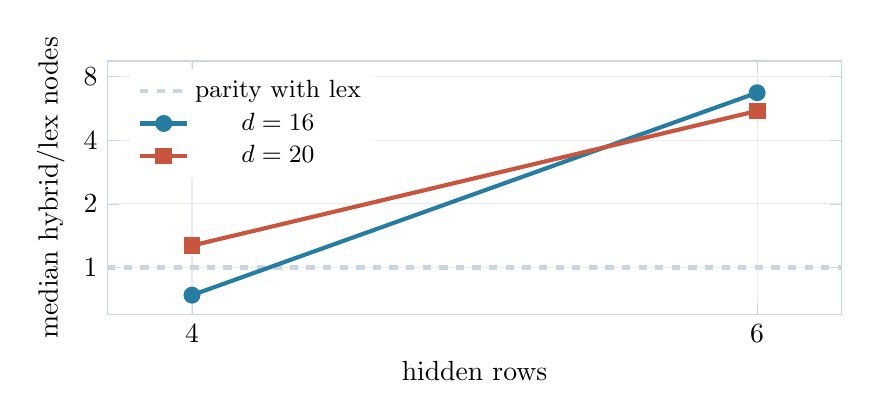
\begin{tikzpicture}
\begin{axis}[
  width=0.90\linewidth,
  height=4.8cm,
  ymode=log,
  log basis y={2},
  xmin=3.7,xmax=6.3,
  ymin=0.6,ymax=9.5,
  xtick={4,6},
  ytick={0.5,1,2,4,8},
  yticklabels={$0.5$,$1$,$2$,$4$,$8$},
  xlabel={hidden rows},
  ylabel={median hybrid/lex nodes},
  axis line style={draw=RuleGray},
  tick style={draw=RuleGray},
  grid=major,
  grid style={draw=RuleGray!45},
  legend style={draw=none,fill=white,font=\small,at={(0.03,0.97)},anchor=north west},
  every axis plot/.append style={line width=1.5pt,mark size=2.3pt}
]
\addplot[color=RuleGray,dashed,domain=3.7:6.3] {1};
\addlegendentry{parity with lex}
\addplot[color=SignalBlue,mark=*] coordinates {(4,0.74) (6,6.72)};
\addlegendentry{$d=16$}
\addplot[color=SoftRed,mark=square*] coordinates {(4,1.27) (6,5.51)};
\addlegendentry{$d=20$}
\end{axis}
\end{tikzpicture}
\caption{Depth reversal at $b=8$.  The order-$20$, six-row point uses only the $39$ jointly solved pairs and should be read with its one-sided failures in \cref{tab:closure}.}
\label{fig:reversal}
\end{figure}

The more constructive stress test makes the comparison concrete.  From two seed rows at order $12$, lexicographic and hybrid policies both solve all $15$ presentations.  Lexicographic search needs a median $74$ nodes and $0.063$ seconds; the hybrid needs $1{,}385$ nodes and $1.083$ seconds.  Their paired median ratios are $7.59$ for nodes and $15.21$ for time.  Randomized-tie all-pair ordering solves only $3$ of $15$ runs.

\takeaway{The pairwise regional state contains genuine search information relative to weak policies, but its local advantages do not compose with depth.  The strongest controlled baseline is not random; it is the structure-aligned lexicographic order.}

\section{Why the correct marginal becomes the wrong action}

Three mechanisms reconcile the notes.  First, the regional law describes a continuation drawn from a matrix already known to be complete.  Search visits counterfactual states, changing its own state distribution after every choice.  Second, \eqref{eq:score} adds dependent pairwise marginals.  A block can satisfy each debt plausibly while their joint arrangement leaves no completion.  Third, lexicographic order appears aligned with regular small-order representatives or implicit algebraic structure that the marginal score does not encode.  The last explanation is suggested by the evidence, not proved by it.

The result is neither ``there is no local structure'' nor ``prediction cannot help search.''  The all-pair policy usually improves on balance-only and stochastic controls, and one shallow condition beats lexicographic search.  The narrower conclusion is that next-region likelihood is the wrong terminal target for a greedy constructor.  The next score should estimate \eqref{eq:value}, bounded look-ahead survival, or residual value beyond a strong structural baseline.

This also sets an engineering gate.  Transferring the present policy into mature SAT/CAS machinery is not justified until a controlled residual policy yields robust node reduction and credible wall-clock gain against lexicographic or solver-native activity.  Promising experiments include predicting survival to depth $h$, estimating the number of feasible descendants, selecting among algebraic templates, and learning when the structural baseline is likely to fail.

\section{Conclusion}

The three-note arc now separates three statements that initially looked like one.  A coordinate representation can make individual entries readable.  The invariant constraint state can make regional summaries predictable.  Neither fact guarantees that greedily preferred regions compose into a complete matrix.

That separation is the useful result.  Hadamard matrices reveal how global order can make local summaries predictable without making local decisions wise.  The constraint state tells us what the next region should look like; the remaining challenge is to tell which plausible region can belong to a complete whole.

\paragraph{Reproducibility.}
The repository contains the exact solver, unit tests, commands, seeds, source and solution digests, raw run tables, paired summaries, budgets, and environment metadata for all four retained result families.  Budget-limited jobs are never labeled unsatisfiable.

\bibliographystyle{plainnat}
\bibliography{references}

\end{document}
